\chapter{Vectors, Matrices \& Determinants}

Welcome to Mathematics for Data Science 2! Linear algebra is the foundational mathematical backbone of modern Machine Learning, Artificial Intelligence, and Data Science. From storing high-dimensional feature spaces to computing neural network transformations and performing dimensionality reduction, vectors and matrices are the fundamental building blocks.

\section{Vectors in $\mathbb{R}^n$}

A \textbf{Vector} in $n$-dimensional real space $\mathbb{R}^n$ is an ordered sequence of $n$ real numbers, written as a column matrix:
$$\mathbf{v} = \begin{bmatrix} v_1 \\ v_2 \\ \vdots \\ v_n \end{bmatrix} \in \mathbb{R}^n$$

\begin{definitionbox}{Vector Operations}
For vectors $\mathbf{u}, \mathbf{v} \in \mathbb{R}^n$ and scalar $c \in \mathbb{R}$:
\begin{itemize}
    \item \textbf{Vector Addition:} $\mathbf{u} + \mathbf{v} = \begin{bmatrix} u_1 + v_1 \\ u_2 + v_2 \\ \vdots \\ u_n + v_n \end{bmatrix}$
    \item \textbf{Scalar Multiplication:} $c \mathbf{v} = \begin{bmatrix} c v_1 \\ c v_2 \\ \vdots \\ c v_n \end{bmatrix}$
    \item \textbf{Dot Product:} $\mathbf{u} \cdot \mathbf{v} = \mathbf{u}^T \mathbf{v} = \sum_{i=1}^{n} u_i v_i = u_1 v_1 + u_2 v_2 + \dots + u_n v_n$
\end{itemize}
\end{definitionbox}

\begin{intuitionbox}{Geometric Vector Addition (Parallelogram Law)}
While vector addition is just adding numbers row-by-row, geometrically it represents combining two movements in space. If you walk along vector $\mathbf{u}$ and then walk along vector $\mathbf{v}$, your total displacement is $\mathbf{u} + \mathbf{v}$. This forms the diagonal of the parallelogram created by $\mathbf{u}$ and $\mathbf{v}$.
\begin{center}
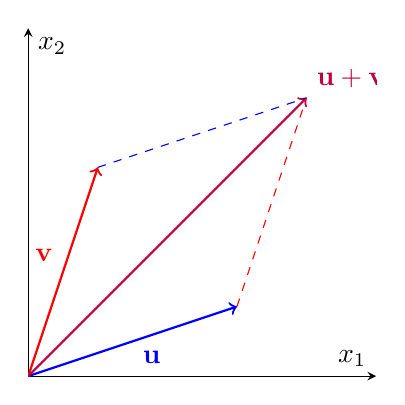
\begin{tikzpicture}
\begin{axis}[
    width=6cm, height=6cm,
    axis lines=middle,
    xmin=0, xmax=5,
    ymin=0, ymax=5,
    xlabel={$x_1$}, ylabel={$x_2$},
    ticks=none
]
% Vector u
\draw[->, thick, blue] (axis cs:0,0) -- (axis cs:3,1) node[midway, below right] {$\mathbf{u}$};
% Vector v
\draw[->, thick, red] (axis cs:0,0) -- (axis cs:1,3) node[midway, above left] {$\mathbf{v}$};
% Vector u+v
\draw[->, thick, purple] (axis cs:0,0) -- (axis cs:4,4) node[above right] {$\mathbf{u}+\mathbf{v}$};
% Dashed lines for parallelogram
\draw[dashed, blue] (axis cs:1,3) -- (axis cs:4,4);
\draw[dashed, red] (axis cs:3,1) -- (axis cs:4,4);
\end{axis}
\end{tikzpicture}
\end{center}
\end{intuitionbox}

\textbf{Data Science Relevance:} In data science, a sample (e.g. a user profile with age, income, credit score) is represented as a feature vector $\mathbf{x} \in \mathbb{R}^d$. The linear combination $\mathbf{w}^T \mathbf{x} + b$ forms the prediction score in Linear and Logistic Regression!

\begin{videocard}{IITM BS Lecture: Vectors}{https://www.youtube.com/watch?v=1So2VV9Tm_A}
Official lecture defining vector spaces, geometric interpretations, and algebraic operations in $\mathbb{R}^n$.
\end{videocard}

\section{Matrices and Matrix Operations}

A \textbf{Matrix} $A \in \mathbb{R}^{m \times n}$ is a rectangular array of $m$ rows and $n$ columns:
$$A = \begin{bmatrix} a_{11} & a_{12} & \dots & a_{1n} \\ a_{21} & a_{22} & \dots & a_{2n} \\ \vdots & \vdots & \ddots & \vdots \\ a_{m1} & a_{m2} & \dots & a_{mn} \end{bmatrix}$$

\begin{theorembox}{Matrix Multiplication}
If $A \in \mathbb{R}^{m \times k}$ and $B \in \mathbb{R}^{k \times n}$, their product $C = AB \in \mathbb{R}^{m \times n}$ has entries:
$$c_{ij} = \sum_{p=1}^{k} a_{ip} b_{pj}$$
Matrix multiplication is associative $(AB)C = A(BC)$ and distributive, but \textbf{NOT commutative} ($AB \neq BA$ in general).
\end{theorembox}

\begin{intuitionbox}{Matrix Multiplication as Geometric Transformation}
Matrix multiplication isn't just an arbitrary set of dot products---it's a geometric transformation of space!
\begin{itemize}
    \item When you multiply a vector $\mathbf{v}$ by a matrix $A$ ($A\mathbf{v}$), the matrix $A$ grabs the vector and rotates, scales, or shears it to a new location in space.
    \item When you multiply two matrices together ($C = AB$), you are composing two transformations. First apply transformation $B$, then apply transformation $A$.
    \item Because doing Transformation $B$ then $A$ is usually different than doing $A$ then $B$, matrix multiplication is \textbf{not commutative} ($AB \neq BA$).
\end{itemize}
\end{intuitionbox}

\begin{videocard}{IITM BS Lecture: Matrices}{https://www.youtube.com/watch?v=rnIDlZnrCc0}
Official lecture explaining matrix algebra, transposition $A^T$, symmetric matrices ($A = A^T$), and matrix-vector products.
\end{videocard}

\section{Systems of Linear Equations}

A system of $m$ linear equations in $n$ variables $x_1, x_2, \dots, x_n$ can be compactly written in matrix form:
$$A \mathbf{x} = \mathbf{b}$$
where $A \in \mathbb{R}^{m \times n}$ is the coefficient matrix, $\mathbf{x} \in \mathbb{R}^n$ is the vector of unknowns, and $\mathbf{b} \in \mathbb{R}^m$ is the target output.

\begin{definitionbox}{Types of Solutions}
Every linear system $A \mathbf{x} = \mathbf{b}$ has either:
\begin{enumerate}
    \item Exactly \textbf{one unique solution} (consistent, non-singular).
    \item \textbf{Infinitely many solutions} (consistent, dependent).
    \item \textbf{No solution} (inconsistent, parallel constraints).
\end{enumerate}
\end{definitionbox}

\begin{videocard}{IITM BS Lecture: Systems of Linear Equations}{https://www.youtube.com/watch?v=WzR4NKeLHMY}
Official lecture introducing linear systems, augmented matrices $[A \mid \mathbf{b}]$, and geometric interpretations of solutions.
\end{videocard}

\section{Determinants}

The \textbf{Determinant} $\det(A)$ or $|A|$ is a scalar value associated with a square matrix $A \in \mathbb{R}^{n \times n}$ that measures the scaling factor of transformation area/volume.

\begin{formulabox}{Determinant Computation ($2 \times 2$ and $3 \times 3$)}
For $A = \begin{bmatrix} a & b \\ c & d \end{bmatrix}$:
$$\det(A) = ad - bc$$
For $A = \begin{bmatrix} a & b & c \\ d & e & f \\ g & h & i \end{bmatrix}$, expanding along the first row:
$$\det(A) = a(ei - fh) - b(di - fg) + c(dh - eg)$$
\textbf{Invertibility Criterion:} Matrix $A$ is invertible ($A^{-1}$ exists) if and only if $\det(A) \neq 0$.
\end{formulabox}

\begin{videocard}{IITM BS Lecture: Determinants (Parts 1 \& 2)}{https://www.youtube.com/watch?v=A3fxp49I4U8}
Official lectures explaining cofactor expansion, properties of determinants, and invertibility conditions.
\end{videocard}

\newpage
\section{Practice Exercises}
\textit{Detailed step-by-step solutions are available in the Appendix.}

\begin{enumerate}
    \item \textbf{Vector Dot Product \& Angle:} Given vectors $\mathbf{u} = \begin{bmatrix} 2 \\ 3 \\ -1 \end{bmatrix}$ and $\mathbf{v} = \begin{bmatrix} 1 \\ -2 & 4 \end{bmatrix}^T$:
    \begin{enumerate}
        \item Compute the dot product $\mathbf{u} \cdot \mathbf{v}$.
        \item Compute the norms $\|\mathbf{u}\|$ and $\|\mathbf{v}\|$.
    \end{enumerate}

    \item \textbf{Matrix Multiplication:} Given matrices:
    $$A = \begin{bmatrix} 1 & 2 \\ 3 & 4 \end{bmatrix}, \quad B = \begin{bmatrix} 0 & -1 \\ 2 & 5 \end{bmatrix}$$
    Compute $AB$ and $BA$. Verify that $AB \neq BA$.

    \item \textbf{Matrix-Vector System Formulation:} Convert the linear system:
    $$\begin{aligned}
    2x_1 + 3x_2 - x_3 &= 7 \\
    4x_1 - x_2 + 2x_3 &= 3 \\
    -x_1 + 5x_2 + 3x_3 &= 10
    \end{aligned}$$
    into the matrix form $A \mathbf{x} = \mathbf{b}$ and write down the augmented matrix $[A \mid \mathbf{b}]$.

    \item \textbf{Determinant Calculation:} Calculate the determinant of the $3 \times 3$ matrix:
    $$M = \begin{bmatrix} 3 & 1 & 2 \\ 0 & 4 & 5 \\ 1 & 2 & 1 \end{bmatrix}$$
    Is matrix $M$ invertible?

    \item \textbf{Data Science Application (Covariance Matrix Determinant):} In multivariate statistics, the determinant of a $2 \times 2$ Covariance Matrix $\Sigma = \begin{bmatrix} \sigma_1^2 & \sigma_{12} \\ \sigma_{12} & \sigma_2^2 \end{bmatrix}$ represents total generalized variance. Given $\sigma_1^2 = 4$, $\sigma_2^2 = 9$, and covariance $\sigma_{12} = 3$, calculate $\det(\Sigma)$.
\end{enumerate}